\addcontentsline{toc}{chapter}{Введение}
\chapter*{Введение}

Большое количество современных систем являются беспроводными. Простота развертывания, мобильность, относительно низкая
стоимость - вот основные преимущества беспроводных систем. Количество мобильных устройств (телефоны, планшетные компьютеры
и т.д.) с каждым годом стремительно растет, только мобильных телефонов в 2011 году было 5.6 миллиарда, что обеспечило покрытие 79.86\%
\cite{wiki_mobilenum} населения земли. Технологии беспроводной связи глубоко проникли во все сферы жизни общества:
обеспечение безопасности с помощью датчиков радиочастотной идентификации (RFID - Radio Frequency IDentification),
предоставление доступа в интернет по технологиями сетей третьего поколения (3G - third generation), сетям на базе стандарта IEEE 802.11 (Wi-Fi),
сотовая связь по различным технологиям (GSM - Global System for Mobile Communications, CDMA - Code Division Multiple Access, DAMPS - Digital Advanced Mobile Phone Service).
Некоторые из этих систем строятся на основе методики
расширения спектра, которая отвечает современным требованиям по мощности сигнала и по безопасности передаваемых
данных. В основе таких систем лежат шумоподобные (широкополосные) сигналы (ШПС). Вместе с тем растут требования к таким
системам. Применение ШПС ставит ряд специфических задач по обработке информации, обусловленных особенностями ШПС.
Решение этих задач приводит к усложнению методов обработки ШПС.

Внедрение новых технологий требует увеличение полосы частот. Разнообразие технологий беспроводной передачи данных среди
гражданских и военных систем ведет к перегрузке каналов связи и все более высоким требованиям к скорости передачи
данных. Поэтому применение систем передачи информации с ШПС становится все более неизбежным.

Принимая во внимание географические размеры России и стратегическую важность обладания собственными системами спутникового
позиционирования, правительство Российский Федерации уделяет особое внимание разработке собственной системы
глобального спутникового позиционирования ГЛОНАСС. Обладание собственными технологиями системы спутниковой навигации (СНС), государство может обезопасить
себя в случае военных конфликтов от ограничения применения американской СНС Navstar GPS в зоне конфликта.

Разработка систем, позволяющих работать с несколькими различными СНС, позволит повысить точность определения координат
в сложных условиях города. Сложность детектирования сигнала и определения координат обусловлена наличием плотной
застройки многоэтажными зданиями. В городских условиях задача подавления интерференционной помехи становится особенно
актуальной. Спектр интерференционной помехи не является белым, а фильтрация и компенсация цветного шума
требует разработки специальных алгоритмов.

Новые цифровые процессоры позволяют применять подходы, которые еще 10-15 лет назад были бесперспективными.
В данной работе развиваются подходы на основе построения параметрической модели ШПС. Невозможность использования
методов, требующих вычислений с высокой точностью в приемниках реального времени,
10-15 лет назад была обусловлена слабой производительностью процессоров и микроконтроллеров, а также существенной
стоимостью процессоров с модулем для операций с числами с плавающей точкой. Современное развитие цифровых технологий делает 
возможным применение параметрических методов оценки спектра взамен традиционного подхода основанного на непараметрического
анализа спектра.

Основы теории систем связи с ШПС были заложены в работах \mbox{В.А. Котельникова} и \mbox{К. Шеннона}.
В России исследованиями в этой области занимаются \mbox{В.И. Борисов}, \mbox{В.Б. Пестряков}, \mbox{В.И. Журавлев}, \mbox{М.И. Жодзишский},
\mbox{Б.И. Шахтарин}, \mbox{Л.Е.  Варакин}, \mbox{В.Е. Гантмахер} и др.

Изначально методы расширения спектра применялись при разработке военных систем управления и связи \cite{sklyar}.
К концу второй мировой войны расширение спектра применялось в радиолокации для борьбы с преднамеренными помехами, а
впоследствии развитие данной технологии объяснялось желанием создать помехоустойчивые системы связи.
В конце 40-х - начале 50-х годов прошлого века \mbox{Мортимер Рогофф}, сотрудник Международной Телефонной и Телеграфной Корпорации (США) (ITT),
провёл эксперимент по передаче информации при помощи псевдошумового сигнала \cite{sklyar}, среди отечественных ученых
в середине 30-х годов прошлого века работу об основах кодового разделения каналов написал \mbox{Д.В. Агеев.}
Первые разработки таких систем относились к военным отраслям. Данный факт объясняется рядом свойств, которыми обладают
ШПС, привлекательными для разработчиков СПИ специального назначения, в числе которых — сложность перехвата заложенной в них информации,
высокая помехоустойчивость, а также трудность обнаружения факта работы передатчика. В процессе исследований расширенному спектру
нашлось и другое применение - снижение плотности энергии, высокоточная локация, использование при множественном доступе
\cite{sklyar}.

Системы связи с широкополосными сигналами занимают особое место среди прочих современных систем передачи информации.
Высокая помехозащищенность под воздействием сильных помех, кодовое разделение большого количества абонентов, прием
информации с высокой достоверностью - отличительные особенности таких систем. Эти свойства систем с ШПС были известны и ранее, но
уровень и стоимость элементной базы с одной стороны, и низкий уровень интерференционных помех с другой стороны, не приводили к острой необходимости развития систем данного класса.
Однако усовершенствование элементной базы привело к широкому распространению данного вида сигналов. В настоящее время ШПС применяются в системах спутниковой навигации,
системах сотовой связи и др \cite{varakin-book}.

Отношение сигнал/шум (ОСШ) на входе приемника может быть очень низким. Для обеспечения высокой помехозащищенности 
в таких случаях используются ШПС с большими и сверхбольшими базами.

К созданию сложных широкополосных сигналов (СШС) привело решение ряда проблем при развитии систем передачи данных.
Первая проблема встала при разработке новых радиолокационных систем. Для дальнейшего их развития необходимо было 
разрешить несколько групп противоречивых требований: требование высокой разрешающей способности по дальности и требование к малой дальности обнаружения
целей в импульсных РЛС, требование точного измерения скорости и требование к высокому разрешению по дальности, требование к
увеличению дальности и ограничению пиковой мощности \cite{gantmaher-book}. Решение данных задач было предложено
Ф. Вудвардом. Им было показано, что дополнительным параметром в таких системах может быть форма сигнала. Длительность сигнала
может быть больше - настолько больше, насколько это необходимо для обеспечения энергетических требований, а требование
разрешения по дальности и точности измерений определяются шириной полосы сигнала. Данные требования обеспечиваются
путем сжатия импульса на стороне приемника. Вудворд сформулировал основные принципы ШПС: произведение эффективной полосы частот
радиосигнала на его длительность должен быть существенно больше единиц ${FT>>1}$, внутренняя структура сигнала
должна быть такой, чтобы обеспечить возможность приемнику сжатие распределенного во времени сигнала в короткий импульс,
соответствующий полосе ${F}$ \cite{gantmaher-book}.

В \cite{gantmaher-book} показана связь пропускной способности канала с понятием ШПС. При ${R_e<<1}$ можно записать:
\begin{equation}
	%\label{eq:shennon_cdma}
	FT = \frac{1}{\log(1+R_e)}, \nonumber
\end{equation}
где ${R_e}$ - ОСШ, ${F}$ - эффективная полоса частот, ${T}$ - длительность.

Стоить отметить, что при ${R_e<<1}$, левая часть данного выражения стремится к бесконечности, а значит
ШПС позволяет обеспечить теоретически неограниченную достоверность передачи информации. Второе важное свойство
ШПС - способность работать "под шумами". Что обеспечивает скрытность
передачи информации, а с другой высокую степень уплотнения каналов связи и, как следствие, решение современных проблем
с перегруженностью каналов связи.

В процессе диссертационного исследования используется подход программного приемника (Software Defined Receiver - SDR)
для оценки параметров ШПС \cite{akos-book, grayver-book, pany-book}. Особенностью данного подхода является реализация алгоритмов
обработки сигнала на системах общего назначения. Автор использует математический пакет MATLAB. Богатая библиотека подпрограмм, удобный интерфейс
и возможность вести разработку на ПК делают выбор подхода практически безальтернативным в процессе научного исследования.
Традиционные подходы к реализации программного приемника СНС Navstar GPS отражены в \cite{akos-book, tsui}. 

Как уже было отражено выше, ШПС применяется во многих системах. Особенный интерес у автора вызывает СНС Navstar GPS. Этому есть две причины:
\begin{itemize}
	\item ШПС, используемый в СНС Navstar GPS, является "типовым" в системах данного класса, для расширения спектра в данной системе используется ПСП Голда \cite{gold-ieee};
	\item данные СНС Navstar GPS находятся в открытом доступе и их можно использовать в процессе эксперимента для подтверждения результатов имитационного
		моделирования и теоретического исследования.
\end{itemize}

Интересными представляются исследования в области детектирования и оценки
частоты ШПС с применением теории хаоса (осциллятора Дуффинга) \cite{chaos_cambridge, chaos_chen, chaos_huang, chaos_wang}. Преимуществом
данного подхода является то, что свойства осциллятора позволяют детектировать сигналы с экстремально низким ОСШ.

Осциллятор Дуффинга \cite{kobilkina_phd, sidorkina_phd, rukovica_phd} с гармоническим внешним воздействием может быть описан уравнением:
\begin{equation}
	\label{eq:duffing}
	mx'' + cx' + k_{1}x + k_{2}x^3 = F_{0}\cos(\omega{t}),
\end{equation}
где $m$ - масса, $c$ - коэффициент диссипации, $x$ - состояние осциллятора, $k_1$ и $k_2$ - линейный и нелинейный коэффициенты соответственно,
$F_{0}\cos(\omega{t})$ - внешнее воздействие.

Подробно уравнение (\ref{eq:duffing}) рассмотрено в \cite{chaos_neimark_landa}.
Для использования осциллятора Дуффинга с целью оценки параметров ШПС была предложена усовершенствованная форма \cite{chaos_song, chaos_chen}:
\begin{equation}
	\label{eq:duffing_gps}
	x'' +cx' - x^3 + x^5 = \gamma\cos(\omega{t}) + (\gamma_{x}\cos(\omega_{x}) + n(t)).
\end{equation}

Можно переписать динамическую систему (\ref{eq:duffing_gps}) в виде:
\begin{equation}
	\label{eq:duffing_gps_2}
	\left\{
	\begin{aligned}
		y(t) & = x'(t); \\
		y'(t) & =  -cx' + x^3 - x^5 + \gamma\cos(\omega{t}) + (\gamma_{x}\cos(\omega_{x}) + n(t)),
	\end{aligned}
	\right.
\end{equation}
где ${n(t)}$ - аддитивный белый гауссовский шум (АБГШ), имеющий нулевое среднее  значение и КФ ${R_n(\tau) = \frac{N_0}{2} \delta(\tau)}$,
а ${N_0}$ - односторонний энергетический спектр.

Пример фазового портрета системы (\ref{eq:duffing_gps_2}) при ${\omega=\omega_{x}}$ изображен на \mbox{Рис. \ref{pic:duffing_sync}},
фазовый портрет системы в режиме хаоса изображен на \mbox{Рис. \ref{pic:duffing_chaos1}} и \mbox{Рис. \ref{pic:duffing_chaos2}}.
\begin{figure}[h]
	\center\scalebox{0.5}{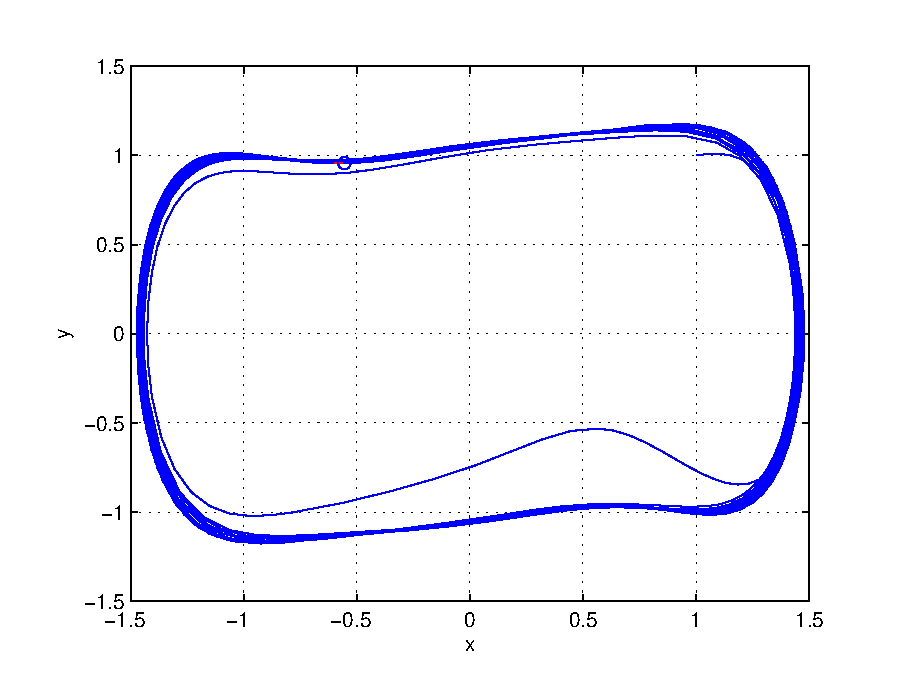
\includegraphics[width=1\linewidth]{duffing_sync.eps}}
	\caption{Фазовый портрет при ${\omega =\omega_{x}}$}
	\label{pic:duffing_sync}
\end{figure}
\begin{figure}[h]
	\center\scalebox{0.5}{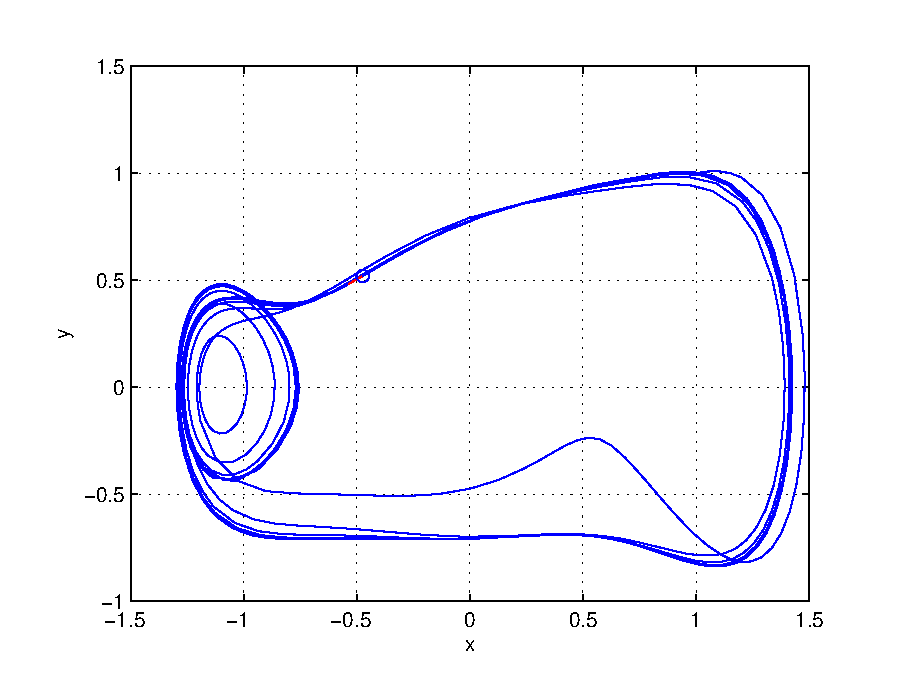
\includegraphics[width=1\linewidth]{duffing_chaos1.eps}}
	\caption{Фазовый портрет при ${\omega < \omega_{x}}$}
	\label{pic:duffing_chaos1}
\end{figure}
\begin{figure}[h]
	\center\scalebox{0.5}{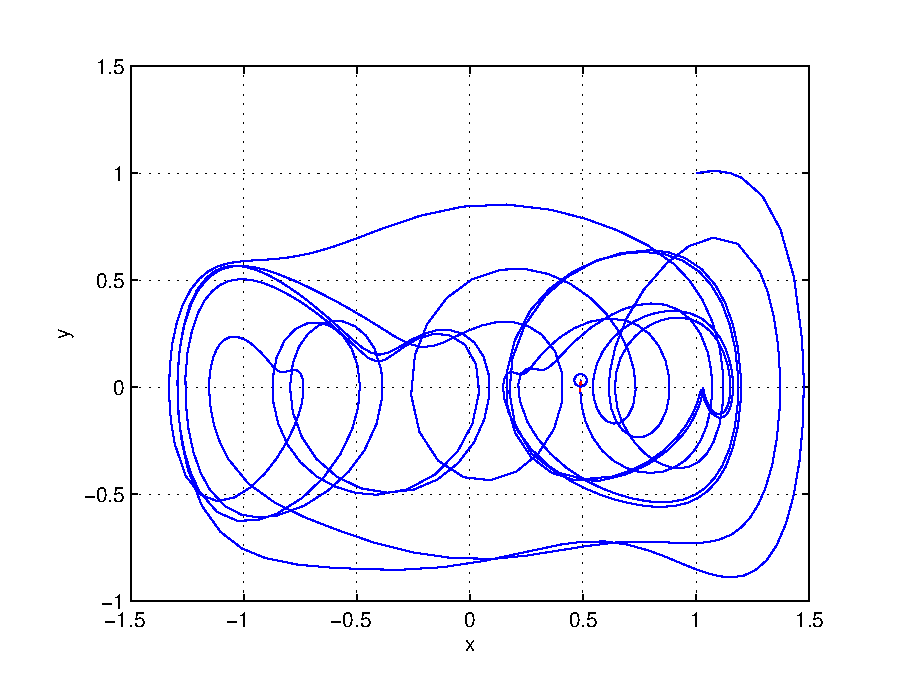
\includegraphics[width=1\linewidth]{duffing_chaos2.eps}}
	\caption{Фазовый портрет при ${\omega > \omega_{x}}$}
	\label{pic:duffing_chaos2}
\end{figure}
Для Рис. \ref{pic:duffing_sync} В качестве параметров уравнения применялись: $c = 0.5$, $\gamma=\gamma_{x}=0.36$, ${\omega=1}$.

Часто для определения параметров режимов хаотической динамики системы применяются показатели Ляпунова.
По их значениям можно определить в каком состоянии находится система.
%Если система находится
%в стабильном состоянии линии фазовой траектории будут близко прилегать одна к другой, в противном
%случае система находится в состоянии хаоса.
Детектор с применением показателя Ляпунова представлен на \mbox{Рис. \ref{pic:chaos_lyapunov}}.
\begin{figure}[h]
	\center\scalebox{0.7}{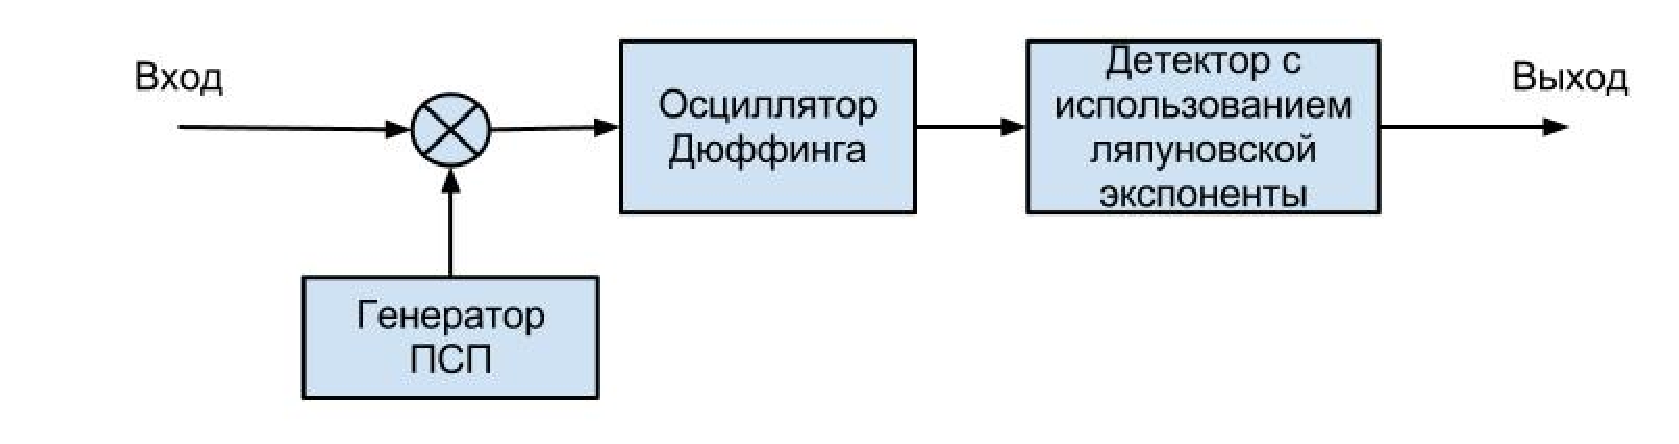
\includegraphics[width=1\linewidth]{Chaos_detector_Lyapunov.eps}}
	\caption{Схема детектора, основанного на показателе Ляпунова для осциллятора Дуффинга}
	\label{pic:chaos_lyapunov}
\end{figure}

В статье \cite{chaos_chen} предложен усовершенствованный метод, базирующийся на вычислении дисперсии
фазовой траектории. Действительно, на Рис. \mbox{\ref{pic:duffing_chaos1}} и \mbox{Рис. \ref{pic:duffing_chaos2}} видно, что когда система находится в хаотическом состоянии значение
дисперсии по координате ${x}$ больше, чем соответствующее значение в состоянии $\omega = \omega_{x}$.
На основе этого была предложена усовершенствованная схема детектора сигнала - \mbox{Рис. \ref{pic:chaos_energy_detector}}.
\begin{figure}[h]
	\center\scalebox{0.7}{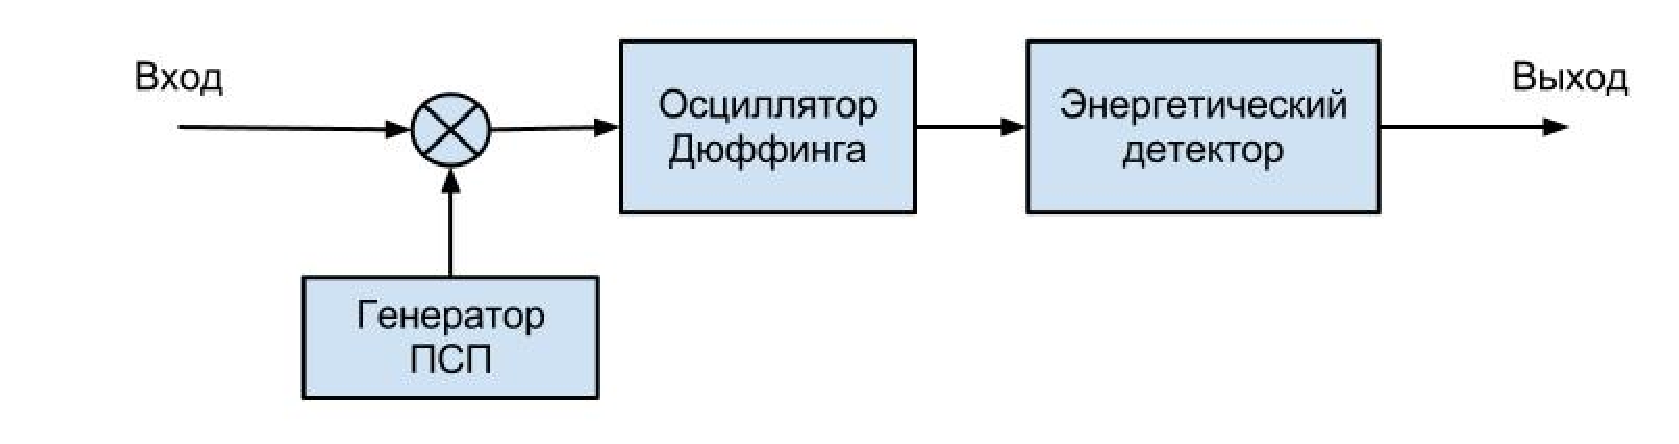
\includegraphics[width=1\linewidth]{chaos_detector.eps}}
	\caption{Схема энергетического детектора для осциллятора Дуффинга}
	\label{pic:chaos_energy_detector}
\end{figure}

Вместе с тем, из-за высокой чувствительности хаотических режимов к изменению параметров и начальных условий системы, использование данного подхода
в реальных приемниках затруднительно. Таким образом данное направление является в настоящее время скорее теоретическим, чем практическим.

В работах \cite{hos_petropulu, hos_zhao} предложено использовать статистики высоких порядков (СВП) для подавления шума и оценки
сигналов с низким уровнем ОСШ.

Математический аппарат статистик высоких порядков (СВП или HOS - Higher-order statistics)
для исследования непричинных, причинных и нестабильных
(систем с не минимальной фазой) и негауссовых сигналов впервые был предложен в \cite{hos_petropulu} в 1993 году.
Этот метод позволяет не только подавлять цветной гауссовский шум, но также в некоторых случаях подавлять
цветной негауссовский шум. В работе \cite{hos_zhao} был предложен метод оценки параметров ШПС с использованием СВП.

Интересная группа алгоритмов основывается на информационной избыточности ШПС, например, \cite{phd_che}. В данной
группе алгоритмов используется механизм появления нескольких точек на основном пике КФ, описанный в \cite{kaplan}. Пример
изображен на \mbox{Рис. \ref{pic:sec1_peak_tcd}}.
\begin{figure}[h]
	\center\scalebox{1}{\includegraphics[width=1\linewidth]{corr_peak_tcd.eps}}
	\caption{Идеальная КФ ШПС с отмеченными точками возможного обнаружения}
	\label{pic:sec1_peak_tcd}
\end{figure}

На \mbox{Рис. \ref{pic:sec1_peak_tcd}} изображен пик КФ с несколькими точками. Две точки находятся выше порога ${\Pi=0.5}$.

В работе \cite{phd_che} рассмотрено создание субоптимального обнаружителя на основе информационной избыточности ШПС.
Получена целевая функция для системы синхронизации в целом и намечены дальнейшие пути развития данного направления.

Более традиционные подходы оценки параметров ШПС сигналов с низким уровнем ОСШ рассмотрены в монографии \cite{ziedan-book}.
В данной монографии рассматриваются как методы детектирования и оценки параметров ШПС, основанные на когерентном накоплении, так и эффективные
системы слежения за частотой и фазой ПСП.

Так же публикуются работы по выбору порога в алгоритмах захвата ШПС. Например, в работах \cite{2max_ieee, 2max_article} представлен алгоритм
\textquotedblleft{Peak-finding algorithm}\textquotedblright,
в данной работе введем перевод -
\textquotedblleft{Алгоритм нахождения пика}\textquotedblright (АНП). 

Предложенный в работах алгоритм можно разбить на несколько шагов:
\begin{itemize}
	\item[Шаг 1.] Подсчитать КФ, используя БПФ.
	\item[Шаг 2.] Найти главный пик КФ, найти второй пик КФ, найти среднее значение КФ.
	\item[Шаг 3.] Нормализовать полученные значения относительно главного пика КФ.
	\item[Шаг 4.] Если (максимум КФ - среднее) > ${\Pi_1}$ и (максимум КФ - 
		второй максимум КФ) > ${\Pi_2}$, тогда принимается решение о наличии сигнала в принимаемой смеси. 
\end{itemize}

В статье \cite{2max_ieee} предложены следующие значения для порогов: \mbox{${\Pi_1} = 0.3$ дБ} и  \mbox{${\Pi_2} = 0.15$ дБ.}
Так же авторы предлагают итерационную процедуру для нахождения фазы ПСП и частоты смещения Доплера:
\begin{itemize}
	\item[Шаг 1] Начать вычисление с 1 мс.
	\item[Шаг 2] Получить результаты АНП.
	\item[Шаг 3] Если фаза ПСП и частота не могут быть найдены, увеличить время интегрирования сигнала.
		Использовать следующие значения для интегрирования: 1мс -> 10мс -> 50мс -> 100мс -> 200мс -> 500мс -> 1000мс.
\end{itemize}

Таким образом интерес исследователей и разработчиков к СПИ с ШПС в последнее время огромен. Это в первую очередь связано с их
практически безальтернативностью  в таких приложениях как радиолокация, спутниковая навигация, мобильная связь и др. При проектировании таких систем
для выделения данных из потока необходимо иметь точно синхронизированную копию ПСП, которая была использована
при модулировании сигнала на передающей стороне. Для достижения синхронизма на стороне приемника необходимо
устранить неопределенность в двух областях: неопределенность по частоте и неопределенность по фазе (задержке) ПСП.
Неопределенность по фазе ПСП обусловлена неопределенностью в расстоянии между передатчиком и приемником. Неопределенность
по частоте обусловлена доплеровским эффектом, а также нестабильностью опорных генераторов в
передатчике и приемнике. После устранения неопределенности по частоте, для достижения точной синхронизации
начинается процесс слежения за частотой. Неопределенность по фазе ПСП устранить, не используя полный перебор,
невозможно в силу корреляционных свойств ПСП. Таким образом можно заключить, что задача быстрого и эффективного
поиска и оценки информационных параметров ШПС является актуальной.

%%%%%%%%
{\bf{Цель и задачи диссертации}}

Целью диссертационной работы является разработка и анализ алгоритмов оценки информационных параметров сигнала в системах с CDMA на основе
параметрического метода оценки частоты на фоне аддитивного белого гауссовского шума (АБГШ) и интерференционной помехи, с возможностью реализации на современной элементной базе.

Для достижения поставленной цели в диссертации решаются следующие задачи:
\begin{enumerate}
	\item {Разработка алгоритма оценки информационных параметров для одного источника сигнала в CDMA-системах на фоне АБГШ с использованием методов параметрической идентификации.}
	\item {Адаптация и усовершенствование итеративного алгоритма вычисления оценки автокорреляционной функции (АКФ) для использования при обработке CDMA-сигнала в приемниках реального времени.}
	\item {Разработка комплексированного алгоритма оценки информационных параметров CDMA-сигнала на фоне АБГШ и интерференционной помехи, основанного на алгоритмах Delay and Multiply Approach (DMA), а также усовершенствованном алгоритме итеративной оценки автокорреляционной функции и авторегрессионной (АР) модели второго порядка.}
	\item {Сравнительный анализ разработанных алгоритмов с типовыми решениями в области оценки информационных параметров сигнала используемых в CDMA-системах.}
	\item {Полунатурное моделирование с использованием оригинальной аппаратной платформы на реальных данных CDMA-системы Navstar GPS, а также полунатурное моделирование на данных, полученных из внешних источников.}
\end{enumerate}

{\bf{Общая методика исследований}}

Разрабатываемые в работе алгоритмы оценки информационных параметров ШПС основываются на параметрическом моделировании. Методы исследований основаны на теории вероятностей,
статистической теории радиотехнических систем, теории цифровых систем. Для решения задач используется численное и полунатурное моделирование. Для полунатурного моделирования
используется подход реализации программного приемника (SDR - Software Defined Receiver) и получения данных для эксперимента при помощи оригинальной аппаратной платформы.

{\bf{Научная новизна результатов}}
\begin{enumerate}
	\item {На основе теории параметрической идентификации автором разработан алгоритм оценки информационных параметров сигнала в CDMA-системах.}
	\item {Предложен алгоритм компенсации окрашенного шума на основе итеративного вычисления АКФ для получения несмещенной оценки частоты с использованием параметрического метода оценки спектра.}
	\item {Предложен усовершенствованный итеративный алгоритм вычисления оценки АКФ в базисе Фурье для использования в приемниках реального времени.}
	\item {Предложен способ комплексирования алгоритмов оценки фазы псевдослучайной последовательности (ПСП) DMA, усовершенствованного алгоритма итеративного вычисления оценки АКФ и параметрического метода оценки спектра в задаче оценки информационных параметров сигнала в CDMA-системах.}
\end{enumerate}

{\bf{Практическая ценность}}
\begin{enumerate}
	\item {Усовершенствован итеративный алгоритм вычисления оценки АКФ. Оптимизация вычислительных затрат позволяет использовать данный усовершенствованный алгоритм в приемниках реального времени.}
	\item {Усовершенствованный алгоритм итеративного вычисления оценки АКФ позволяет повысить ОСШ при оценке АКФ, а также снизить влияние окрашенного шума на точность оценки частоты при использовании АР модели.}
	\item {Разработанный комплексированный алгоритм оценки информационных параметров CDMA-сигнала позволяет существенно снизить вычислительные затраты.}
	\item {Созданный программно-аппаратный стенд для экспериментального исследования систем цифровой связи с использованием технологии CDMA позволяет подтвердить практическую реализуемость разработанных алгоритмов.}
\end{enumerate}

{\bf{Апробация результатов}}
Результаты диссертации прошли апробацию на 7-ой Всероссийской конференции «Радиолокация и радиосвязь» (Москва 2013 г.); Международной конференции «Радиоэлектронные устройства и системы для инфокоммуникационных технологий - РЕС-2013» (Москва 2013 г.); V Международной студенческой научно-практической конференции «Интеллектуальный потенциал XXI века: ступени познания» (Новосибирск 2011 г.).

{\bf{Внедрение результатов работы:}}
\begin{enumerate}
	\item {Результаты диссертации внедрены в экспериментальном программно-аппаратном обеспечении филиала «Самсунг Электроникс Ко., Лтд», что подтверждено актом о внедрении.}
	\item {Результаты диссертации использованы в НИР «Фундаментальные проблемы создания АУИС», шифр «КЕДР-5», ГР№: 01200964825.}
	\item {Результаты диссертации использованы в учебном процессе на кафедрах «Автономные информационные и управляющие системы» МГТУ им. Н.Э. Баумана, и
		«Управление и моделирование систем» Московского Государственного Университета Приборостроения и Информатики, что подтверждено актами об использовании.}
\end{enumerate}

{\bf{Объем и структура диссертации}}

Диссертация состоит из введения, четырех глав, заключения и списка литературы. Общий объем составляет \_\_\_ страниц, включающих 24 страниц приложения, 52 иллюстрации,
\_\_ таблицы и список литературы из 62 наименований.

{\bf{Положения, выносимые на защиту}}
\begin{enumerate}
	\item {Алгоритм оценки информационных параметров CDMA-сигнала на фоне АБГШ на основе АР-модели принимаемого сигнала.}
	\item {Усовершенствованный итеративный алгоритм вычисления оценки АКФ для повышения ОСШ и подавления интерференционной помехи в задаче оценки информационных параметров CDMA-сигнала.}
	\item {Комплексированный алгоритм оценки информационных параметров CDMA-сигнала на фоне интерференционной помехи и шума на основе алгоритмов: DMA, усовершенствованного итеративного алгоритма вычисления оценки АКФ и АР-модели принимаемого сигнала.}
	\item {Результаты анализа точности, вычислительных затрат разработанных алгоритмов, а также сравнительный анализ с типовыми алгоритмами.}
\end{enumerate}

%%%%%%
\clearpage
